% Fluxion-Tide: the landscape. Compile with: xelatex landscape.tex (twice)
\documentclass[10pt,a4paper]{article}
\usepackage[a4paper,margin=2.1cm,top=2.3cm,bottom=2.3cm]{geometry}
\usepackage{fontspec}
\setmainfont{Inter}[UprightFont=*-Regular, BoldFont=*-SemiBold, ItalicFont=*-Italic, BoldItalicFont=*-SemiBoldItalic,
  Extension=.otf, Path=/usr/share/fonts/opentype/inter/, Scale=0.95]
\newfontfamily\display{InterDisplay}[UprightFont=*-SemiBold, BoldFont=*-Bold, Extension=.otf, Path=/usr/share/fonts/opentype/inter/]
\newfontfamily\displaylight{InterDisplay}[UprightFont=*-Light, Extension=.otf, Path=/usr/share/fonts/opentype/inter/]
\setmonofont{DejaVu Sans Mono}[Scale=0.82]
\usepackage{amsmath,amssymb}
\usepackage{xcolor,graphicx,booktabs,tabularx,array,enumitem,titlesec,fancyhdr,microtype}
\usepackage[most]{tcolorbox}
\usepackage{tikz}
\usetikzlibrary{arrows.meta,positioning,shapes.geometric,calc,fit,backgrounds}
\usepackage[hidelinks]{hyperref}
\usepackage{caption}
\usepackage{float}
\newcolumntype{Y}{>{\raggedright\arraybackslash}X}

% ---------------- colours ----------------
\definecolor{ink}{HTML}{0B0B0B}
\definecolor{ink2}{HTML}{52514E}
\definecolor{muted}{HTML}{8A8984}
\definecolor{rule}{HTML}{E4E3DF}
\definecolor{brand}{HTML}{2A78D6}
\definecolor{brandd}{HTML}{184F95}
\definecolor{brandl}{HTML}{EAF2FC}
\definecolor{orange}{HTML}{EB6834}
\definecolor{orangel}{HTML}{FDF0EA}
\definecolor{aqua}{HTML}{1BAF7A}
\definecolor{aqual}{HTML}{E8F7F1}
\definecolor{amber}{HTML}{C98500}
\definecolor{amberl}{HTML}{FDF5E3}
\definecolor{violet}{HTML}{6250D6}
\definecolor{violetl}{HTML}{EFEDFB}
\definecolor{redl}{HTML}{FCECEC}
\definecolor{red}{HTML}{C93B3A}
\color{ink}

% ---------------- layout ----------------
\setlength{\parindent}{0pt}
\setlength{\parskip}{5pt}
\linespread{1.12}
\setlist{itemsep=2pt,topsep=3pt,leftmargin=14pt}
\setlist[itemize]{label={\color{brand}\textbullet}}
\captionsetup{font={small,color=ink2},labelfont={bf,color=ink},skip=4pt,justification=raggedright,singlelinecheck=false}

\titleformat{\section}{\display\fontsize{19}{23}\selectfont\color{ink}}
  {\colorbox{brand}{\textcolor{white}{\,\thesection\,}}}{10pt}{}[\vspace{-4pt}\textcolor{rule}{\rule{\textwidth}{0.8pt}}]
\titleformat{\subsection}{\display\fontsize{12.5}{15}\selectfont\color{brandd}}{\thesubsection}{8pt}{}
\titleformat{\subsubsection}{\bfseries\color{ink}}{}{0pt}{}
\titlespacing*{\section}{0pt}{6pt}{10pt}
\titlespacing*{\subsection}{0pt}{12pt}{4pt}
\titlespacing*{\subsubsection}{0pt}{8pt}{2pt}

\pagestyle{fancy}\fancyhf{}
\fancyhead[L]{\small\color{muted}Fluxion-Tide \textperiodcentered{} the landscape}
\fancyhead[R]{\small\color{muted}\leftmark}
\fancyfoot[C]{\small\color{muted}\thepage}
\renewcommand{\headrulewidth}{0pt}
\renewcommand{\sectionmark}[1]{\markboth{#1}{}}

% ---------------- boxes ----------------
\newtcolorbox{plain}[1][In plain words]{enhanced,breakable,colback=brandl,colframe=brandl,boxrule=0pt,arc=3pt,
  left=9pt,right=9pt,top=6pt,bottom=6pt,borderline west={2.5pt}{0pt}{brand},
  title={\bfseries #1},coltitle=brandd,attach title to upper,after title={\ \ }}
\newtcolorbox{keep}[1][Keep in mind]{enhanced,breakable,colback=amberl,colframe=amberl,boxrule=0pt,arc=3pt,
  left=9pt,right=9pt,top=6pt,bottom=6pt,borderline west={2.5pt}{0pt}{amber},
  title={\bfseries #1},coltitle=amber!80!black,attach title to upper,after title={\ \ }}
\newtcolorbox{explore}[1][Worth exploring]{enhanced,breakable,colback=aqual,colframe=aqual,boxrule=0pt,arc=3pt,
  left=9pt,right=9pt,top=6pt,bottom=6pt,borderline west={2.5pt}{0pt}{aqua},
  title={\bfseries #1},coltitle=aqua!70!black,attach title to upper,after title={\ \ }}
\newtcolorbox{warn}[1][Watch out]{enhanced,breakable,colback=redl,colframe=redl,boxrule=0pt,arc=3pt,
  left=9pt,right=9pt,top=6pt,bottom=6pt,borderline west={2.5pt}{0pt}{red},
  title={\bfseries #1},coltitle=red,attach title to upper,after title={\ \ }}

% a gap card: #1 number, #2 title, #3 badge colour, #4 badge text
\newtcolorbox{gapcard}[4]{enhanced,breakable,colback=white,colframe=rule,boxrule=0.7pt,arc=4pt,
  left=10pt,right=10pt,top=7pt,bottom=7pt,before skip=8pt,after skip=8pt,
  title={\display\large\textcolor{brand}{#1}\quad #2\hfill\normalfont\scriptsize\textcolor{white}{\colorbox{#3}{\,\textbf{\strut #4}\,}}},
  colbacktitle=white,coltitle=ink,toptitle=3pt,bottomtitle=1pt,titlerule=0pt}
\newcommand{\row}[1]{\par\smallskip\textcolor{brandd}{\small\bfseries\MakeUppercase{#1}}\enspace}

% key number tile
\newcommand{\tile}[3]{%
\begin{tcolorbox}[enhanced,width=\linewidth,colback=#3,colframe=#3,arc=4pt,boxrule=0pt,left=8pt,right=6pt,top=6pt,bottom=6pt,nobeforeafter]
{\display\fontsize{22}{24}\selectfont #1}\par\vspace{2pt}{\small\raggedright\color{ink2}#2\par}
\end{tcolorbox}}

\tikzset{
  node/.style={draw=rule,fill=white,rounded corners=3pt,align=center,font=\small,inner sep=5pt,line width=0.7pt},
  bnode/.style={node,fill=brandl,draw=brand!40},
  onode/.style={node,fill=orangel,draw=orange!50},
  anode/.style={node,fill=aqual,draw=aqua!50},
  vnode/.style={node,fill=violetl,draw=violet!40},
  gnode/.style={node,fill=black!3},
  arr/.style={-{Stealth[length=5pt]},draw=ink2,line width=0.7pt},
  darr/.style={-{Stealth[length=5pt]},draw=muted,line width=0.6pt,dashed},
}

\begin{document}

% =========================================================== TITLE
\begin{titlepage}
\thispagestyle{empty}
\begin{tikzpicture}[remember picture,overlay]
  \fill[brand] (current page.north west) rectangle ([yshift=-8.2cm]current page.north east);
  \begin{scope}[shift={([yshift=-6.6cm]current page.north west)}]
    \draw[white,opacity=0.35,line width=1.1pt,domain=0:21,samples=300,smooth] plot (\x,{0.45*sin(\x*95)+0.25*sin(\x*270)+0.15*\x/21});
    \draw[white,opacity=0.18,line width=0.9pt,domain=0:21,samples=300,smooth] plot (\x,{0.30*sin(\x*95+40)+0.20*sin(\x*270+70)-0.35});
  \end{scope}
  \node[anchor=north west,inner sep=0pt] at ([xshift=2.1cm,yshift=-1.9cm]current page.north west)
    {\begin{minipage}{16cm}\raggedright\color{white}
     {\displaylight\fontsize{13}{16}\selectfont FLUXION-TIDE \textperiodcentered{} RESEARCH NOTES\par}
     \vspace{10pt}
     {\display\fontsize{34}{38}\selectfont The landscape\par}
     \vspace{8pt}
     {\displaylight\fontsize{15}{19}\selectfont Where we stand, where the points are, what the generator\newline is missing, and how we find out why the model fails\par}
     \end{minipage}};
\end{tikzpicture}
\vspace*{7.6cm}

{\small\color{ink2} Prepared for Naresh \textperiodcentered{} 25 October 2026 \textperiodcentered{} ft3\_main (29M), fev-bench, TIME, synthetic generator clean2}

\vspace{14pt}
\begin{minipage}[t]{0.235\linewidth}\tile{43.8}{our fev-bench skill (groups); the leader has 51.8}{brandl}\end{minipage}\hfill
\begin{minipage}[t]{0.235\linewidth}\tile{69\%}{of a 22M model's gap comes from tasks with covariates}{orangel}\end{minipage}\hfill
\begin{minipage}[t]{0.235\linewidth}\tile{7.4\%}{of our training lanes are targets with known covariates}{amberl}\end{minipage}\hfill
\begin{minipage}[t]{0.235\linewidth}\tile{132k}{series in the planned benchmark-free dev slice}{aqual}\end{minipage}

\vspace{18pt}
{\display\Large What this document says, in five sentences}
\vspace{4pt}
\begin{enumerate}[leftmargin=18pt,itemsep=4pt]
\item We are 8 skill points behind the fev-bench leader and 23rd of 40 on TIME; model size is not the lever (our 100M was no better than the 30M, and a 5M model beats us).
\item For models at our level, most of the missing points sit in a few dozen tasks, and most of those come with covariates (weather, prices, holidays, opening days).
\item Our generator is strong on seasonality, repetition and textbook dynamics, but weak where real use lives: covariates that drive a target, real calendars, history that shows a cycle only once or twice, breaks, and true gaps.
\item We now have a benchmark-free catalog of 377 real datasets to check every change against, and a method to find \emph{why} a forecast failed, not just that it did.
\item The plan: cheap switches first, then covariate scenarios with a causal-graph generator and a calendar engine, tested at 5M before a single confirmation at 30M.
\end{enumerate}

\vfill
\begin{tcolorbox}[colback=black!2,colframe=black!2,arc=3pt,boxrule=0pt,left=8pt,right=8pt]
\small\color{ink2}\textbf{How to read this.} Blue boxes explain an idea in plain words. Amber boxes are rules to keep. Green boxes are directions worth exploring. Every number comes from our own runs, the published fev-bench result files, or the project notes; estimates are marked as estimates.
\end{tcolorbox}
\end{titlepage}

\tableofcontents
\thispagestyle{fancy}
\newpage

% =========================================================== 1
\section{Where we stand}

Our best model, \texttt{ft3\_main} (29M parameters, trained only on synthetic data), scores \textbf{43.78} on fev-bench with its covariate (group) mode on and 42.09 with it off. The leader, TimeRSI-1.5, scores \textbf{51.8}. On TIME we are 23rd of 40 at a normalised MASE of 0.680; Chronos-2 is at 0.662 and Timestral-5M at 0.652.

\begin{figure}[H]
\centering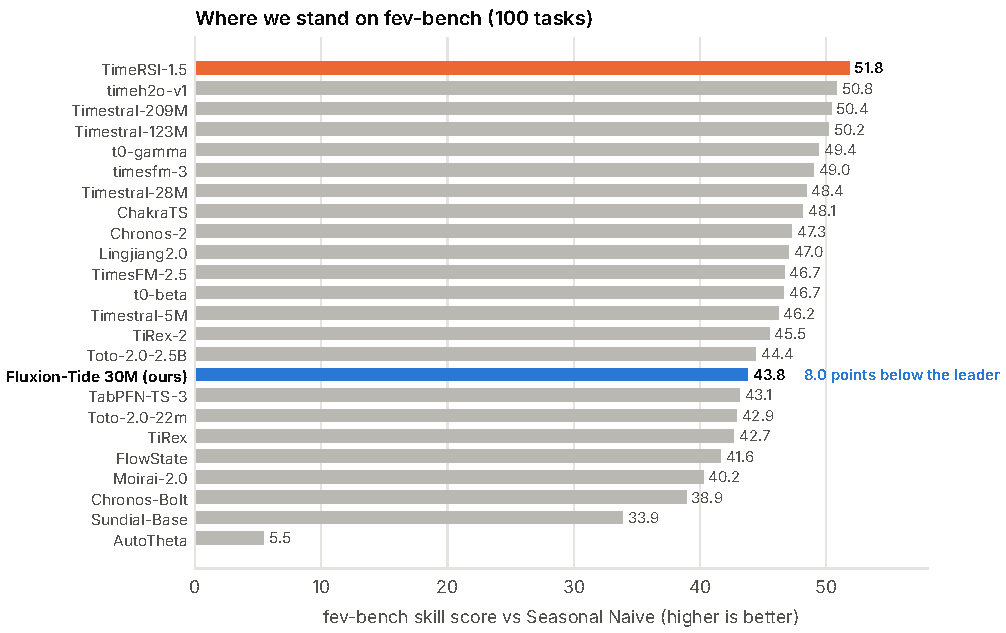
\includegraphics[width=0.92\linewidth]{figs/f1_fev_board.pdf}
\caption{fev-bench skill scores computed from the result files published in the fev repository (higher is better). Our row is the owner's own scoring of ft3\_main with groups on; the other rows use the published per-task files. Naive and five models with missing tasks are left out.}
\end{figure}

\begin{plain}
A \textbf{skill score} says how much smaller a model's error is than a very simple forecaster (Seasonal Naive: ``repeat the last cycle''). A skill of 44 means our error is about 56\% of Seasonal Naive's, averaged in a way that treats every task equally. Going from 43.8 to 51.8 means cutting our error by about 15\% across the board, which is a lot.
\end{plain}

\begin{figure}[H]
\centering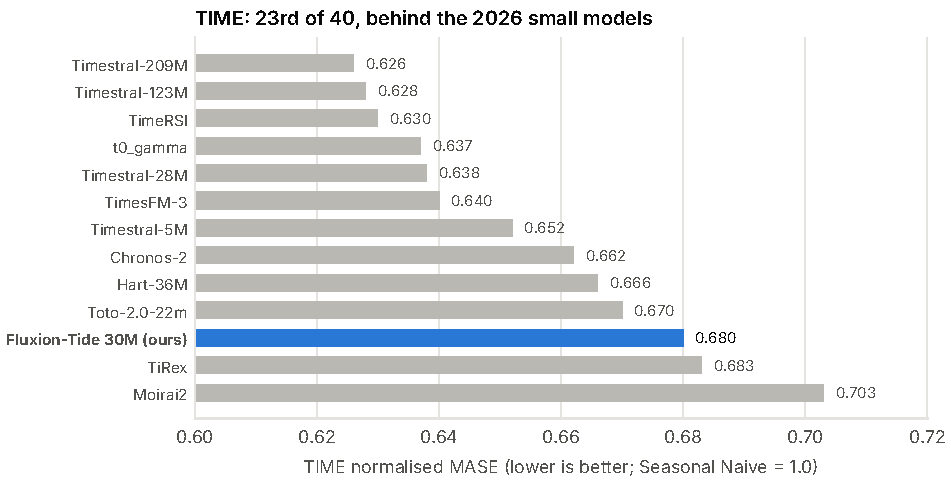
\includegraphics[width=0.86\linewidth]{figs/f5_time_board.pdf}
\caption{TIME (50 fresh datasets, 98 tasks) normalised MASE, excerpt of the 40-model board from our notes (TIME\_FULL\_LEADERBOARD). Lower is better.}
\end{figure}

\begin{keep}
\begin{itemize}
\item Against the top models the gap is \textbf{broad}: we beat Chronos-2 on 24\% of TIME tasks and Timestral-28M on 9\%.
\item Size is not the lever: our 100M was $+0.21$ skill over the 30M on fev (not significant), and Timestral-5M beats our 30M on about 90\% of TIME tasks.
\item Real-data post-training gave about $+0.5$ skill, but that pool was 96\% weather. It shows \emph{that} data did not help much, not that real data cannot.
\end{itemize}
\end{keep}

% =========================================================== 2
\section{The three scoreboards}

Three benchmarks decide how a time-series foundation model is judged. They overlap in style but not in data, and each has rules for what may touch training.

\begin{table}[H]
\centering\small
\begin{tabularx}{\linewidth}{>{\bfseries}l Y Y Y}
\toprule
 & TIME & fev-bench & GIFT-Eval (test) \\
\midrule
Size & 39 datasets, 50 dataset/frequency entries, 98 tasks & 100 tasks over 59 dataset configurations & 28 datasets, 97 configurations \\
Character & fresh data (2025), mostly FRED economics, energy, IMOS ocean, Singapore city data, Azure 2019 & energy, retail and cloud heavy; 42-46 tasks give covariates & classic sets: M4, electricity, solar, traffic, ETT, hospital \\
Metric & MASE and CRPS / Seasonal Naive, geometric mean & SQL skill vs Seasonal Naive, win rate & MASE, CRPS ranks \\
How we use it & final check only & final check; per-task files for analysis & not used for selection \\
\bottomrule
\end{tabularx}
\caption{The benchmarks. Lists were read from the benchmark repositories on 25 October 2026 (TIME \texttt{datasets.yaml}, fev \texttt{tasks.yaml}, GIFT-Eval notebooks).}
\end{table}

\begin{plain}[Why this matters]
If a dataset from a benchmark, or the same series published somewhere else, ends up in what we tune on, our score on that benchmark stops meaning anything. Several TIME datasets are FRED republications, so ``FRED'' as a whole is unsafe unless we remove those exact series. The same goes for crypto prices, Singapore weather and PM2.5, EIA crude and product prices, and the 2019 Azure VM trace.
\end{plain}

\begin{keep}[Rules for the scoreboards]
\begin{itemize}
\item Never choose a model, a generator setting or a mix weight by looking at TIME. Keep a count of how many times we look at fev.
\item Tune on the dev catalog (Section~\ref{sec:data}), confirm on a locked part of it, and score fev and TIME at the end.
\item fev differences below about 0.3 skill points are mostly noise; always use paired confidence intervals.
\end{itemize}
\end{keep}

% =========================================================== 3
\section{Where the missing points are}

The published fev result files let us split the gap between a model at our level and the leader, task by task. Two facts stand out.

\begin{figure}[H]
\centering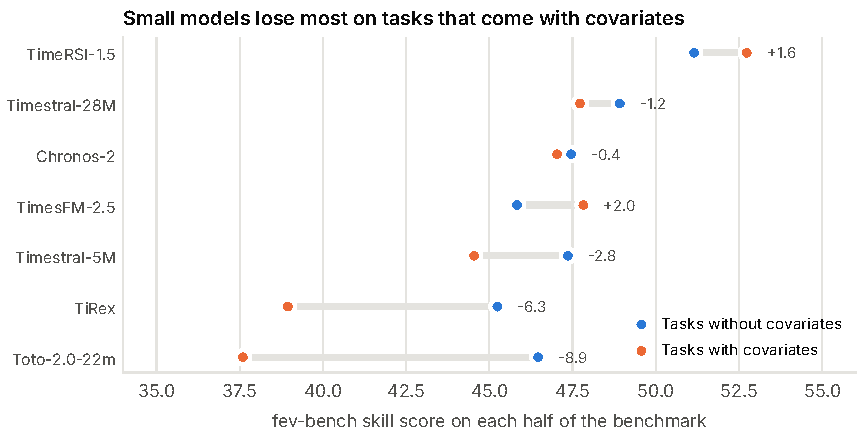
\includegraphics[width=0.92\linewidth]{figs/f2_cov_split.pdf}
\caption{Skill on the tasks without covariates (blue) and with covariates (orange). The number is the difference. Small models fall off sharply when covariates are present; the leader does not.}
\end{figure}

\textbf{Fact one: covariates.} For Toto-2.0-22m, a model at our level, 69\% of the gap to TimeRSI-1.5 comes from the tasks that supply covariates. If it matched the leader on those tasks alone it would score 49.2 instead of 42.9. For Timestral-5M the share is 61\%, for Chronos-2 53\%.

\begin{figure}[H]
\centering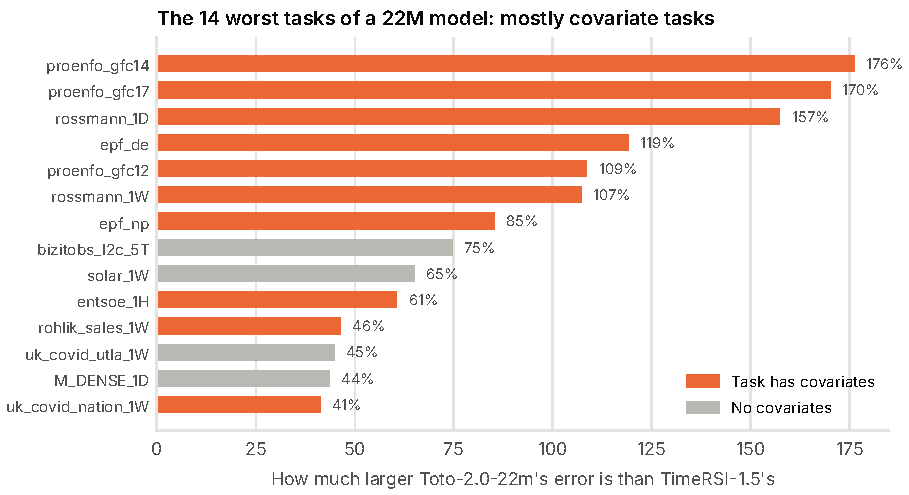
\includegraphics[width=0.92\linewidth]{figs/f4_worst_tasks.pdf}
\caption{The 14 tasks where Toto-2.0-22m is furthest behind the leader. Ten of them come with covariates: GEFCom load with temperature, Rossmann sales with opening days, promotions and holidays, electricity prices with load and wind forecasts, ENTSO-E load with radiation and temperature.}
\end{figure}

\textbf{Fact two: concentration.} Ten tasks hold 42\% of the gap and 25 tasks hold 70\%. We do not need to be a little better everywhere; we need to stop losing badly in a few recognisable places.

\begin{figure}[H]
\centering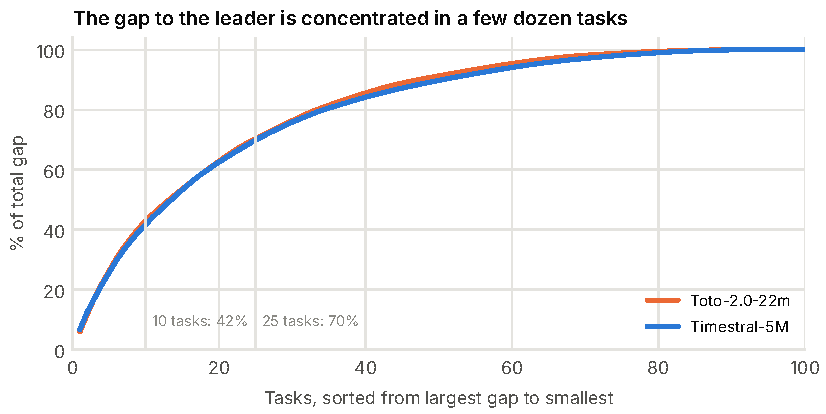
\includegraphics[width=0.92\linewidth]{figs/f3_gap_conc.pdf}
\caption{Cumulative share of the gap to TimeRSI-1.5, tasks sorted from the largest gap down. The two models have almost the same curve.}
\end{figure}

\begin{plain}[What a covariate is]
A covariate is another series that helps explain the one we forecast. Some are \textbf{known in the future} (the temperature forecast, a planned promotion, whether the shop is open, a public holiday); some are only \textbf{known in the past} (yesterday's number of customers). A model that can read them correctly gets a large advantage on exactly the tasks where we lose most.
\end{plain}

\begin{warn}[Not yet measured for us]
These splits use other models' published files. We have not yet run the same split on ft3\_main's own per-task file. Our group mode adds 1.7 skill points (43.78 vs 42.09); Chronos-2 reports about 16\% lower error on known-covariate tasks, our earlier v4 about 4\%. Running the split on our own file is the first thing to do.
\end{warn}

% =========================================================== 4
\section{Our generator today}

ft3\_main learned only from synthetic series. The generator (\texttt{tidemark/real/ft3\_core.py}, profile \texttt{clean2}) draws a base family, then stacks layers on top. I ran it on CPU (2,048 series at each of four lengths) to measure what it actually produces.

\begin{figure}[H]
\centering
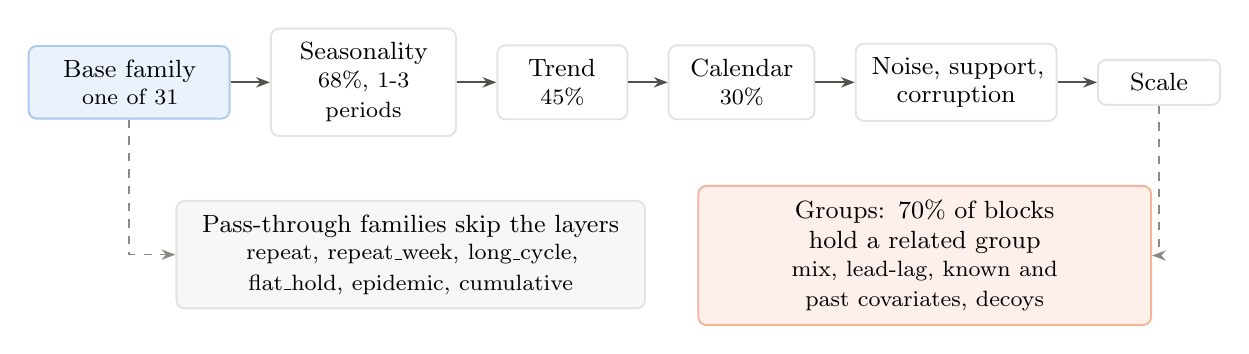
\begin{tikzpicture}[node distance=5mm and 5mm]
\node[bnode,text width=2.2cm] (fam) {Base family\\[-1pt]{\footnotesize one of 31}};
\node[node,right=of fam,text width=2.0cm] (sea) {Seasonality\\[-1pt]{\footnotesize 68\%, 1-3 periods}};
\node[node,right=of sea,text width=1.3cm] (tr) {Trend\\[-1pt]{\footnotesize 45\%}};
\node[node,right=of tr,text width=1.5cm] (cal) {Calendar\\[-1pt]{\footnotesize 30\%}};
\node[node,right=of cal,text width=2.2cm] (noi) {Noise, support,\\[-1pt]corruption};
\node[node,right=of noi,text width=1.2cm] (sc) {Scale};
\node[gnode,below=8mm of sea,xshift=6mm,text width=5.6cm] (pt) {Pass-through families skip the layers\\[-1pt]{\footnotesize repeat, repeat\_week, long\_cycle, flat\_hold, epidemic, cumulative}};
\node[onode,below=8mm of noi,xshift=-4mm,text width=5.4cm] (grp) {Groups: 70\% of blocks hold a related group\\[-1pt]{\footnotesize mix, lead-lag, known and past covariates, decoys}};
\draw[arr] (fam)--(sea); \draw[arr] (sea)--(tr); \draw[arr] (tr)--(cal); \draw[arr] (cal)--(noi); \draw[arr] (noi)--(sc);
\draw[darr] (fam.south) |- (pt.west);
\draw[darr] (sc.south) |- (grp.east);
\end{tikzpicture}
\caption{How one synthetic series is made. Percentages are the share of eligible rows that receive a layer.}
\end{figure}

\begin{figure}[H]
\centering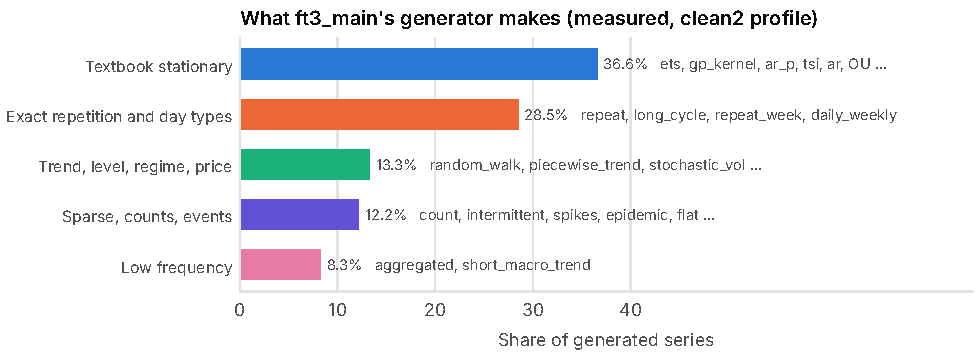
\includegraphics[width=0.92\linewidth]{figs/f6_gen_mix.pdf}
\caption{Share of generated series by role, measured from the family weights of the clean2 profile with the ft3 additions (agg, periods, epidemic, repeat, day types, weekday, yearly).}
\end{figure}

\begin{figure}[H]
\centering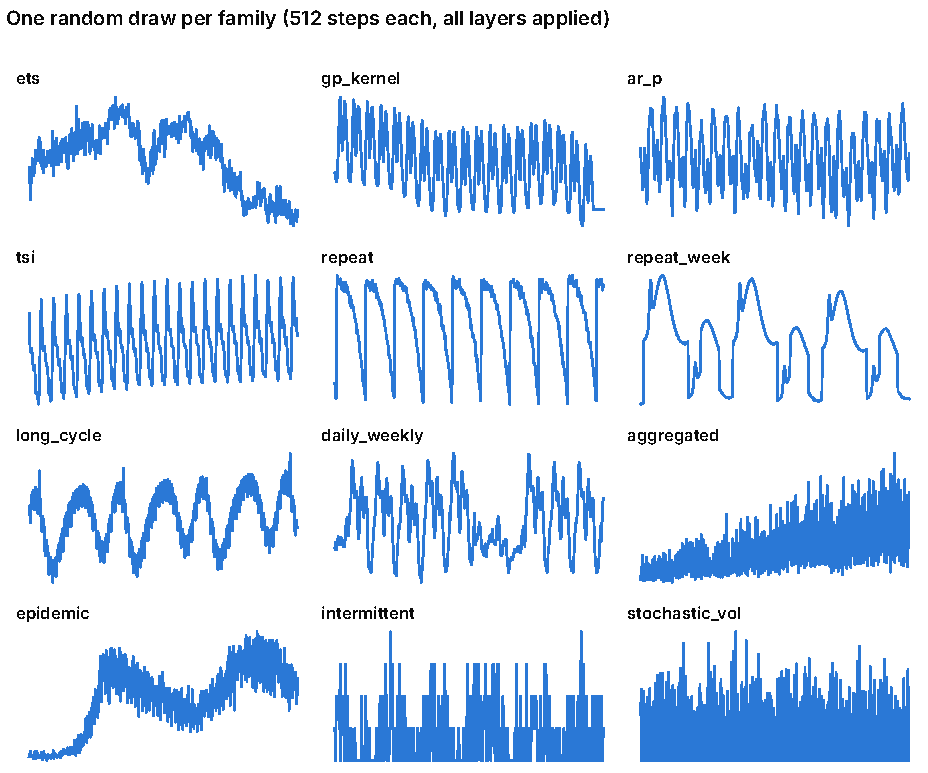
\includegraphics[width=0.94\linewidth]{figs/f8_gallery.pdf}
\caption{One random draw from each of twelve families, after all layers. The generator already covers smooth stationary dynamics, exact repetition, day types, long cycles, aggregation, epidemics, intermittency and volatility.}
\vspace{10pt}
\centering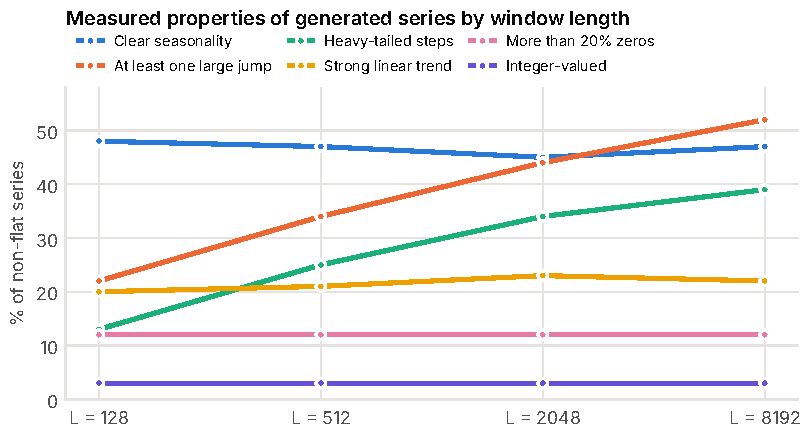
\includegraphics[width=0.92\linewidth]{figs/f7_gen_props.pdf}
\caption{Measured properties by window length (\% of non-flat series). About half the series are clearly seasonal at every length; only 3\% are integer-valued.}
\end{figure}

\begin{plain}[What the generator does well]
It was built against measured fev-bench gaps, round after round: non-sinusoidal seasonal shapes, nested periods, exact repetition at any period, weekday versus weekend profiles, low-frequency series made by aggregating daily ones, epidemic waves, flat series that stay flat, cumulative counters, and covariate groups with decoys and on/off gates. That is why a synthetic-only 29M model is level with TiRex and ahead of every 2024-25 model.
\end{plain}

\begin{keep}[Assumptions in this measurement]
The RUN section that trained ft3\_main is not in the repository, so I used the defaults in \texttt{CONFIG} plus \texttt{yearly} and \texttt{cov\_r3} on (the repo notes say ft3\_main used year generators and round-3 covariates). Print \texttt{torch.load("ft3\_main.pt")["cfg"]} to confirm. The seasonality detector only checks lags up to a third of the window, so it misses long\_cycle's 2-4-cycle periods.
\end{keep}

% =========================================================== 5
\section{What the generator is missing}

Each gap below has four parts: what is missing, the evidence, the change, and how to check it. ``Dev'' names real datasets from our benchmark-free catalog.

\begin{table}[H]
\centering\small
\begin{tabularx}{\linewidth}{c >{\bfseries}Y l l}
\toprule
\# & Gap & Kind of work & Priority \\
\midrule
1 & Covariate realism and volume, with a causal-graph generator & new generators & main bet \\
2 & A real calendar engine & new generator layer & main bet \\
3 & History that shows a cycle only once or twice & reweight + calendar & high \\
4 & Structural breaks and regime change & switch exists, off & quick win \\
5 & Drifting and quasi-periodic cycles & switch exists + one family & quick win \\
6 & True missing values (and an inference bug) & small change & quick win \\
7 & Counts, intermittency, product life cycles & one family & high \\
8 & Hierarchies & group kind & later \\
9 & Nonlinear dynamics (ODE systems) & offline pool & later \\
10 & Financial tails & one family & later \\
\bottomrule
\end{tabularx}
\caption{Summary of the gaps, ranked by expected effect on fev and TIME (judgement informed by the measurements above).}
\end{table}

\begin{gapcard}{1}{Covariate realism and volume}{orange}{MAIN BET}
\row{Missing} A continuous covariate is just another synthetic series, and its effect is a fixed curve (linear, ReLU, tanh, step or V) that never depends on time of day or season. The real patterns that cost the most are not generated as such: temperature driving load differently at each hour; price set by residual load (load minus wind and solar) through a steep supply curve; sales shaped by open days, promotion windows, price and typed holidays; PV output following irradiance with inverter clipping. There are no static or categorical covariates at all, and no generic causal-graph generator of the kind t0 uses.
\row{Evidence} Covariate tasks hold 53-69\% of small models' gap on fev. Our group mode adds only 1.7 points. The holiday-flag probe stayed near 0.05 for every twin arm. Only 7.4\% of training lanes are covariate-driven targets.
\row{Change} Scenario generators that draw a target and its covariates from one mechanism (Section~\ref{sec:designs}), plus a causal-graph generator for breadth. Hand known covariates over with forecast error, raise covariate-driven targets to 20-30\% of lanes, with 1-13 covariates per group.
\row{Check} Dev: EIA-930 load with GHCN or ERA5 temperature; SMARD and ENTSO-E prices with load and renewables (not the EPF countries); PV with NASA POWER irradiance; Paris bike counts with weather; Iowa liquor sales with holidays. Target: at least 10\% lower error with covariates than without, where the mechanism exists.
\end{gapcard}

\begin{gapcard}{2}{A real calendar engine}{orange}{MAIN BET}
\row{Missing} Series have no dates. The calendar layer is a weekend effect plus random holiday days (2\%). Months are 30 steps except in the aggregation family. No moving festivals (Easter, Diwali, Eid moving about 11 days a year, Lunar New Year), no daylight-saving 23- and 25-hour days, paydays, month or quarter ends, school terms, bridge days or the Black Friday to Christmas run-up. The model has no calendar input.
\row{Evidence} Holiday probes near 0.05; Rossmann and Rohlik among the worst fev tasks.
\row{Change} Give each series a start date and a frequency; derive weekdays, months, holidays and school terms from real tables for 15-20 countries (the \texttt{holidays} package would be a new dependency). Apply effects with lead and lag windows. Show the calendar as known covariates in about half the rows and hide it in the rest.
\row{Check} Dev: TSA throughput, Eurocontrol traffic, Iowa liquor, Agmarknet mandi prices (Diwali, monsoon), Seattle library checkouts.
\end{gapcard}

\begin{gapcard}{3}{History that shows a cycle only once or twice}{brand}{HIGH}
\row{Missing} Only long\_cycle (9.5\% of series) shows a long period one to six times. Every other seasonal family needs two or three full cycles in the window; about 94\% of detected seasonal series show eight or more. No ``same weekday last year'' alignment, no partial-cycle history.
\row{Evidence} fev history band 2049+: 0.520 vs Chronos-2 0.479, unchanged in every fine-tune. Year-once probe about 0.1. Patch probe: aligned single-occurrence recall 0.98 (Chronos-2 0.24), improving with size (100M: 0.905), so part of this is model capacity.
\row{Change} long\_cycle to about 15\%, built on the calendar engine (day of year, leap years, weekday drift), mostly in contexts of 2,048 points or more.
\row{Check} Year-once and year-twice probes; dev daily series with 1-3 years of history (national park visits, CTA ridership, GHCN daily, library checkouts).
\end{gapcard}

\begin{gapcard}{4}{Structural breaks and regime change}{aqua}{QUICK WIN}
\row{Missing} The breaks layer exists (level, slope, variance, shock with recovery) but is switched off. Breaks only come through three families (about 6\%). It was tested only inside an all-on run, never alone.
\row{Change} Breaks on at 0.2, with some breaks in the last 10-30\% of the context, plus a collapse-and-partial-recovery shape (2020).
\row{Check} Dev: Google mobility, TSA, Eurocontrol, CTA; GNSS station steps. Probe: a break at a controlled place; does the forecast start from the new level?
\end{gapcard}

\begin{gapcard}{5}{Drifting and quasi-periodic cycles}{aqua}{QUICK WIN}
\row{Missing} Seasonal drift (\texttt{tv\_season}) is off. Nothing generates amplitude and frequency modulation, beats of two close periods, or cycles of irregular length.
\row{Change} Switch it on and add one family: $x(t)=A(t)\,s(\varphi(t))$ with $\varphi(t)=2\pi\int_0^t \mathrm{d}u/P(u)$ and a period that wanders a few percent; beats (tides: 12.42\,h with 12\,h); irregular cycles (sunspots 9-14 years, ENSO 2-7 years).
\row{Check} Dev: NOAA tide gauges, sunspots and F10.7, ENSO indices, BioDare2 circadian data, GNSS annual cycles.
\end{gapcard}

\begin{gapcard}{6}{True missing values}{aqua}{QUICK WIN}
\row{Missing} The corruption layer forward-fills its missing runs, so training never marks a single interior point as missing; only left padding and whole hidden patches are masked.
\row{Bug} The univariate forecast path runs \texttt{y = y[np.isfinite(y)]}: it deletes missing values and joins the pieces, which shifts every cycle after a gap. The group path keeps them masked.
\row{Change} Train with scattered and block gaps marked as unobserved, including periodic ones (nights, weekends, market closures); at inference, keep the positions and mask them.
\row{Check} Count how many fev and TIME contexts contain missing values; dev: OpenAQ, NDBC buoys, USGS gauges.
\end{gapcard}

\begin{gapcard}{7}{Counts, intermittency, product life cycles}{brand}{HIGH}
\row{Missing} About 3\% of series are integer. No launch ramp, maturity, decline or death to zero; no stockouts (zeros that mean ``no stock'', then a rebound).
\row{Change} A demand family: low-count Poisson or negative-binomial draws on a seasonal, promotional intensity, Croston-style gaps between orders, a life-cycle envelope and stockout runs.
\row{Check} Dev: VN1 and VN2 competitions, Predict Future Sales, H\&M, Seattle library, NHS prescribing.
\end{gapcard}

\begin{gapcard}{8-10}{Lower priority}{muted}{LATER}
\row{Hierarchies} Groups mix shared factors but nothing sums: add groups where store series add up to region and total (dev: Iowa liquor by store and county, Eurostat regions).
\row{Dynamics} No ODE systems (Lotka-Volterra, seasonally forced SIR, van der Pol, Duffing). Generate them offline into a pool, since time stepping is sequential.
\row{Finance} Jumps, the leverage effect and business-day gaps. The right forecast is close to naive with honest intervals, so check calibration, not point skill.
\end{gapcard}

% =========================================================== 6
\newpage
\section{Three designs for the main bets}\label{sec:designs}

\subsection{Covariate scenarios}

Each scenario draws the target and its covariates from one mechanism, so the relation the model must learn is the one real data has. The equations are sketches; each parameter is drawn at random per series.

\begin{table}[H]
\centering\small
\renewcommand{\arraystretch}{1.5}
\begin{tabularx}{\linewidth}{>{\raggedright\arraybackslash\bfseries}p{2.6cm} Y >{\raggedright\arraybackslash}p{3.2cm}}
\toprule
Scenario & Mechanism & Real example \\
\midrule
Weather to load & $y_t = b_t + \beta_{h(t)}\max(0, T_t - T_c) + \gamma_{h(t)}\max(0, T_h - T_t) + \varepsilon_t$; temperature $T$ has its own daily and yearly cycle; the hourly weights $\beta_h,\gamma_h$ make heating and cooling act at different hours & GEFCom, ENTSO-E, EIA-930 \\
Residual load to price & $p_t = a + b\, e^{c\,(L_t - W_t - S_t)} + \text{spikes}$; load, wind and solar forecasts given as known covariates with forecast error & electricity price markets \\
Sales & $y_t = o_t\,\big(b_t\,(1+\lambda\,\pi_t - \delta\,\pi_{t-k})\,(p_t/\bar p)^{-\eta}\,H_t\big)$; open flag $o_t$, promotion $\pi_t$ with a post-promotion dip, price elasticity $\eta$, typed holidays $H_t$ & Rossmann, Rohlik, M5-like retail \\
Solar output & $y_t = \min\big(C,\ \eta\, I_t\,(1 - k\,(T_t - 25))\big)$; irradiance $I$ zero at night, clipping at capacity $C$ & PV systems with irradiance forecasts \\
Events to traffic & baseline with day types plus event bumps; event calendar as a known flag & bike counters, transit ridership \\
\bottomrule
\end{tabularx}
\end{table}

\subsection{A causal-graph covariate generator}

Hand-built scenarios give realistic shapes but only for the cases we think of. A random causal graph gives breadth: many shapes of ``this series drives that one'', including series that look related but are not.

\begin{figure}[H]
\centering
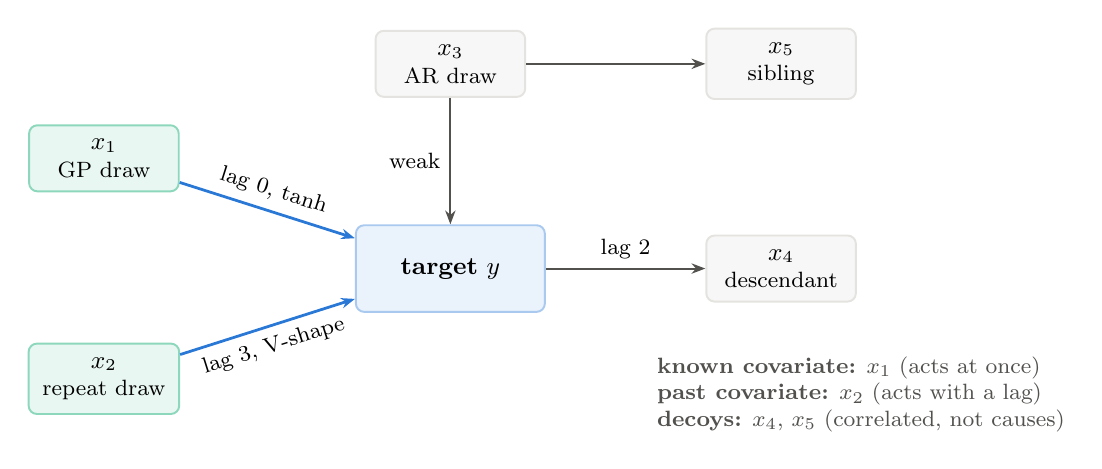
\begin{tikzpicture}[>=Stealth]
\node[anode,minimum width=1.9cm] (a) at (0,1.4) {$x_1$\\[-1pt]{\footnotesize GP draw}};
\node[anode,minimum width=1.9cm] (b) at (0,-1.4) {$x_2$\\[-1pt]{\footnotesize repeat draw}};
\node[gnode,minimum width=1.9cm] (c) at (4.4,2.6) {$x_3$\\[-1pt]{\footnotesize AR draw}};
\node[bnode,minimum width=2.4cm,minimum height=1.1cm] (y) at (4.4,0) {\textbf{target} $y$};
\node[gnode,minimum width=1.9cm] (d) at (8.6,0) {$x_4$\\[-1pt]{\footnotesize descendant}};
\node[gnode,minimum width=1.9cm] (s) at (8.6,2.6) {$x_5$\\[-1pt]{\footnotesize sibling}};
\draw[arr,draw=brand,line width=1pt] (a) -- node[above,font=\footnotesize,sloped]{lag 0, tanh} (y);
\draw[arr,draw=brand,line width=1pt] (b) -- node[below,font=\footnotesize,sloped]{lag 3, V-shape} (y);
\draw[arr] (y) -- node[above,font=\footnotesize]{lag 2} (d);
\draw[arr] (c) -- node[left,font=\footnotesize]{weak} (y);
\draw[arr] (c) -- (s);
\node[font=\footnotesize,text=ink2,align=left,anchor=north west] at (6.9,-1.0) {\textbf{known covariate:} $x_1$ (acts at once)\\\textbf{past covariate:} $x_2$ (acts with a lag)\\\textbf{decoys:} $x_4$, $x_5$ (correlated, not causes)};
\end{tikzpicture}
\caption{One draw. The target's parents become covariates (known if the effect is immediate, past if lagged); a descendant and a sibling go in as decoys that correlate with the target but do not help forecast it.}
\end{figure}

Each node is a base-family series; each edge has a lag and a transfer function:
\[
x_j(t) \;=\; f_j\!\Big(\textstyle\sum_{i \in \mathrm{pa}(j)} w_{ij}\, g_{ij}\big(x_i(t-\ell_{ij})\big)\Big) + \varepsilon_j(t),
\]
with $g$ drawn from linear, saturating, threshold, V-shaped and multiplicative shapes, and $f$ adding the node's own dynamics.

\begin{keep}
t0 (beta and gamma) uses a generator of this kind, but I have not seen an ablation of its effect. Treat it as its own switch, tested alone.
\end{keep}

\subsection{A calendar engine}

\begin{figure}[H]
\centering
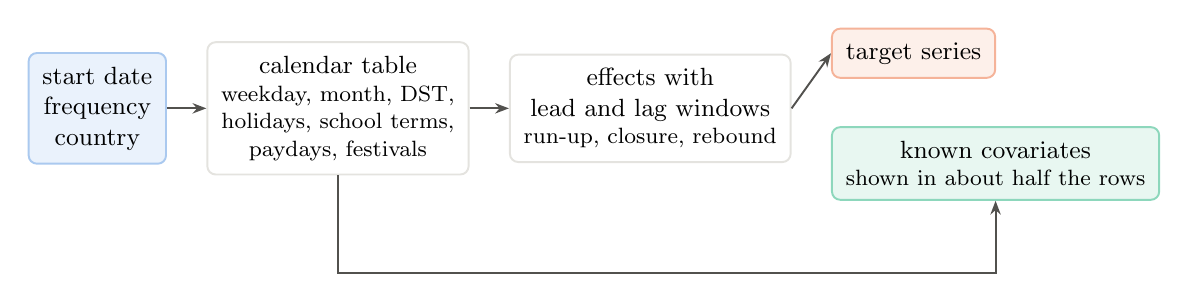
\begin{tikzpicture}[node distance=5mm and 5mm]
\node[bnode] (d) {start date\\frequency\\country};
\node[node,right=of d] (c) {calendar table\\[-1pt]{\footnotesize weekday, month, DST,}\\[-1pt]{\footnotesize holidays, school terms,}\\[-1pt]{\footnotesize paydays, festivals}};
\node[node,right=of c] (e) {effects with\\lead and lag windows\\[-1pt]{\footnotesize run-up, closure, rebound}};
\node[onode,right=of e,yshift=7mm] (t) {target series};
\node[anode,right=of e,yshift=-7mm] (k) {known covariates\\[-1pt]{\footnotesize shown in about half the rows}};
\draw[arr] (d)--(c); \draw[arr] (c)--(e); \draw[arr] (e.east)--(t.west); \draw[arr] (c.south) |- ([yshift=-14mm]e.south) -| (k.south);
\end{tikzpicture}
\caption{The same real calendar shapes the target and, in half of the rows, is handed to the model as known covariates. The model learns both to read calendar inputs and to cope without them.}
\end{figure}

% =========================================================== 7
\section{Real data for checking our work}\label{sec:data}

Tuning the generator against fev or TIME would quietly turn them into training data. So we built a separate catalog of real datasets that are in none of the three benchmarks: \textbf{377 datasets across 26 domains}, from power grids and fuel prices to bacterial growth curves, library checkouts and hard-drive failures.

\begin{figure}[H]
\centering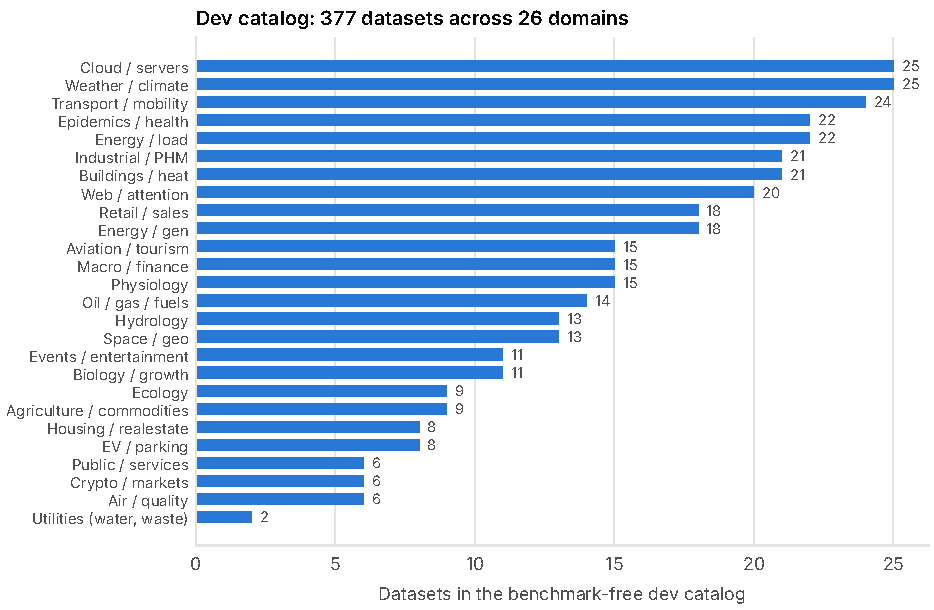
\includegraphics[width=0.9\linewidth]{figs/f9_catalog_domains.pdf}
\caption{Datasets per domain in \texttt{dataset\_catalog\_v2.csv}. 23 catalog entries were removed because they are benchmark data or the same series under another publisher; 29 are kept with named sub-series excluded.}
\end{figure}

\begin{figure}[H]
\centering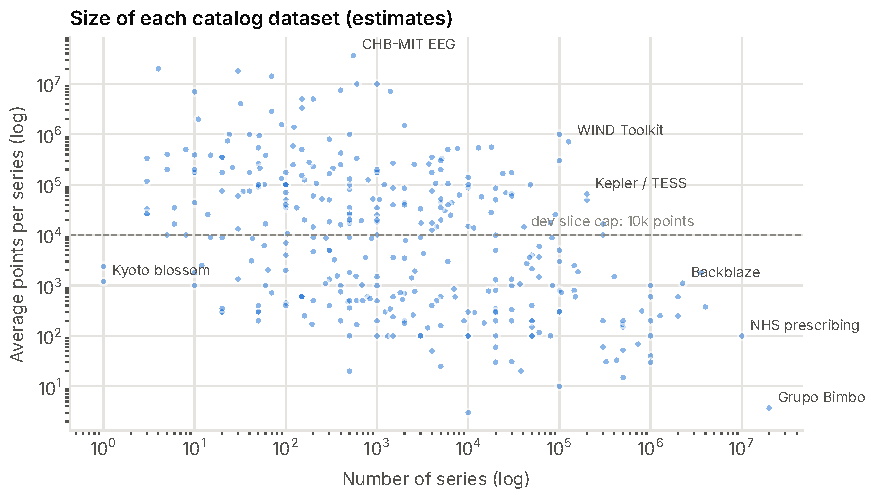
\includegraphics[width=0.9\linewidth]{figs/f10_catalog_sizes.pdf}
\caption{Estimated size of each dataset. The full catalog holds about 62 million series; the planned dev slice takes at most 500 series and 10,000 points from each dataset, about 132,000 series and 650 million points.}
\end{figure}

\begin{figure}[H]
\centering
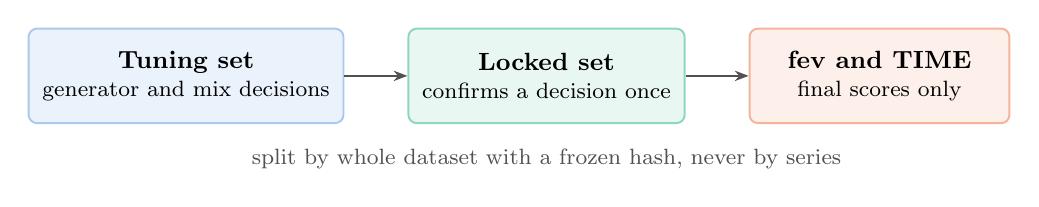
\begin{tikzpicture}[node distance=6mm and 8mm]
\node[bnode,minimum width=3.3cm,minimum height=1.2cm] (dev) {\textbf{Tuning set}\\[-1pt]{\footnotesize generator and mix decisions}};
\node[anode,right=of dev,minimum width=3.3cm,minimum height=1.2cm] (lock) {\textbf{Locked set}\\[-1pt]{\footnotesize confirms a decision once}};
\node[onode,right=of lock,minimum width=3.3cm,minimum height=1.2cm] (fin) {\textbf{fev and TIME}\\[-1pt]{\footnotesize final scores only}};
\draw[arr] (dev)--(lock); \draw[arr] (lock)--(fin);
\node[font=\footnotesize,text=ink2,below=2mm of lock,align=center] {split by whole dataset with a frozen hash, never by series};
\end{tikzpicture}
\caption{Three roles for data. A dataset sits in exactly one role for the whole project.}
\end{figure}

\begin{keep}[About the catalog]
\begin{itemize}
\item Sizes are order-of-magnitude estimates. 148 URLs were confirmed by search; the rest were written from memory, and \texttt{verify\_urls.py} checks them all on your machine.
\item What counts statistically is the number of \emph{datasets}, not series: 100,000 series from one source are still one source. Cap each dataset's share.
\item After downloading, run a series-level check (hashes of values) against the benchmarks, not just a name check.
\end{itemize}
\end{keep}

% =========================================================== 8
\section{Finding out why a forecast fails}

A rising loss tells us \emph{that} something went wrong, not \emph{why}. We find the reason in four steps.

\begin{figure}[H]
\centering
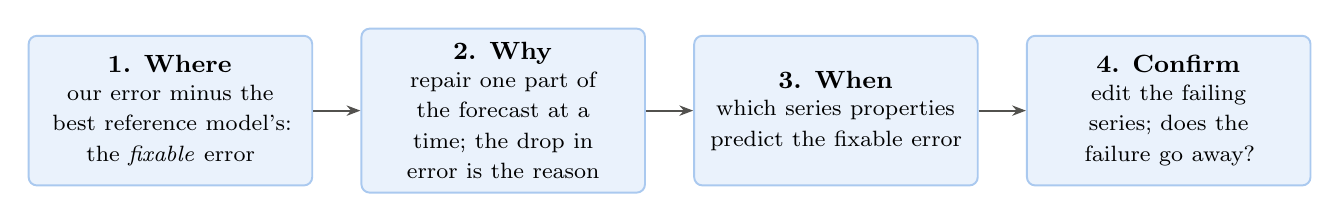
\begin{tikzpicture}[node distance=5mm and 6mm]
\node[bnode,text width=3.25cm,minimum height=1.9cm] (s1) {\textbf{1. Where}\\[-1pt]{\footnotesize our error minus the best reference model's: the \emph{fixable} error}};
\node[bnode,right=of s1,text width=3.25cm,minimum height=1.9cm] (s2) {\textbf{2. Why}\\[-1pt]{\footnotesize repair one part of the forecast at a time; the drop in error is the reason}};
\node[bnode,right=of s2,text width=3.25cm,minimum height=1.9cm] (s3) {\textbf{3. When}\\[-1pt]{\footnotesize which series properties predict the fixable error}};
\node[bnode,right=of s3,text width=3.25cm,minimum height=1.9cm] (s4) {\textbf{4. Confirm}\\[-1pt]{\footnotesize edit the failing series; does the failure go away?}};
\draw[arr] (s1)--(s2); \draw[arr] (s2)--(s3); \draw[arr] (s3)--(s4);
\end{tikzpicture}
\caption{The diagnosis loop. Only a confirmed cause turns into a generator or model change.}
\end{figure}

\subsection{Step 1: fixable error}
For each window we compare our error with the best of several strong models (Chronos-2, TimesFM, Toto, Timestral) and simple baselines. If every model fails, the window is probably unpredictable and we ignore it.
\[
\Delta_{\text{fix}} \;=\; e_{\text{ours}} \;-\; \min_{m\,\in\,\text{references}} e_m .
\]
TIME publishes window-level predictions for every model and fev publishes per-task results, so the references cost nothing.

\subsection{Step 2: attribution by repair}
Take a bad window and replace one part of our forecast with the truth's: its level, its trend, its seasonal amplitude, its phase, its spikes, its interval width. The share of the error that each repair removes is the reason, as a number.

\begin{figure}[H]
\centering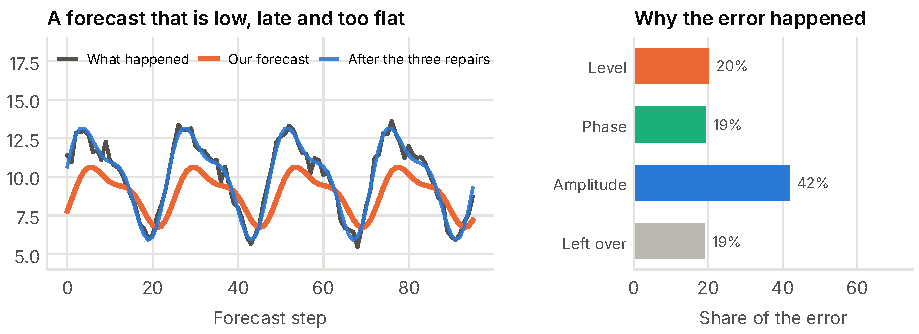
\includegraphics[width=0.94\linewidth]{figs/f11_repair.pdf}
\caption{A worked example on a constructed forecast. The forecast is low, two steps late and too flat. Fixing the level removes 20\% of the error, the phase 19\%, the amplitude 42\%; 19\% is noise that no repair can remove.}
\end{figure}

\begin{plain}[Two failures that look the same]
``It didn't follow the cycle'' can mean the shape is right but late (a \textbf{phase} problem), or the timing is right but the swing is too small (an \textbf{amplitude} problem: the model is hedging). They have different fixes, and the repair split tells them apart.
\end{plain}

\subsection{Step 3: which series properties predict failure}
Compute features per window: period divided by context length, seasonal and trend strength, intermittency, a level shift near the end of the context, whether covariates exist, frequency, length, noise. Then model the fixable error on these features. The output is a short list of rules such as ``we lose when the period is longer than a quarter of the context'' or ``we lose after a late level shift''.

\subsection{Step 4: confirm by intervention}
Edit a failing real series and forecast again: give it more context, remove the shift, rescale it, add or remove a covariate. If the failure disappears, the cause is found. Then build a controlled synthetic probe for it and keep it as a regression test.

% =========================================================== 9
\section{Changes on the model side}

Better data has a ceiling if the model cannot use it. These sit next to the generator work.

\begin{table}[H]
\centering\small
\begin{tabularx}{\linewidth}{>{\raggedright\arraybackslash\bfseries}p{4.2cm} Y l}
\toprule
Change & Why & Cost \\
\midrule
Known covariates see the whole window & today they see one patch ahead; Timestral lets them see the full forecast window and blocks them from reading the target & fine-tune (masks) \\
Static and categorical inputs & store type, region, product category have no way in & small \\
Keep missing positions at inference & the univariate path deletes them and shifts the phase & one line \\
Longer context (32K) and DHF decoding & the 2049+ history band is our weakest & new pre-training \\
21 quantiles, advancing refine frame & better tails and long horizons & fine-tune \\
\bottomrule
\end{tabularx}
\end{table}

% =========================================================== 10
\section{The plan}

\subsection{First experiment: separate data from model}
Timestral-5M's edge is concentrated on covariate tasks (44.5 vs Toto-22m's 37.6, while the two are close without covariates). That could come from data, from covariate attention, or both. Four 5M arms on the same budget answer it:

\begin{table}[H]
\centering\small
\begin{tabularx}{\linewidth}{c Y c c}
\toprule
Arm & What changes & New covariate data & Whole-window covariates \\
\midrule
A & current generator & -- & -- \\
B & covariate scenarios + causal graph & \checkmark & -- \\
C & known covariates see the whole window & -- & \checkmark \\
D & both & \checkmark & \checkmark \\
\bottomrule
\end{tabularx}
\end{table}

Score them on the dev set's covariate datasets and on the covariate probes, then confirm the winner once at 30M (our DHF test showed that 5M results do not always transfer).

\begin{figure}[H]
\centering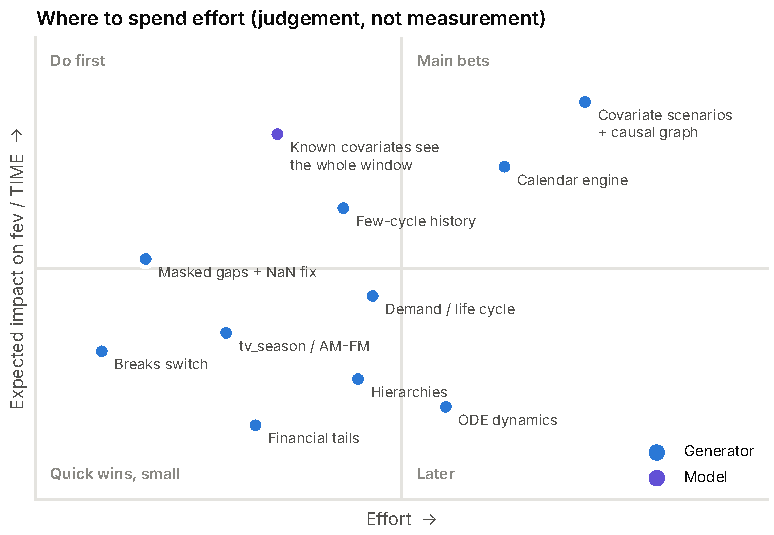
\includegraphics[width=0.86\linewidth]{figs/f12_priorities.pdf}
\caption{Where effort should go. Positions are judgement, informed by the measurements in this document.}
\end{figure}

\subsection{Order of work}
\begin{figure}[H]
\centering
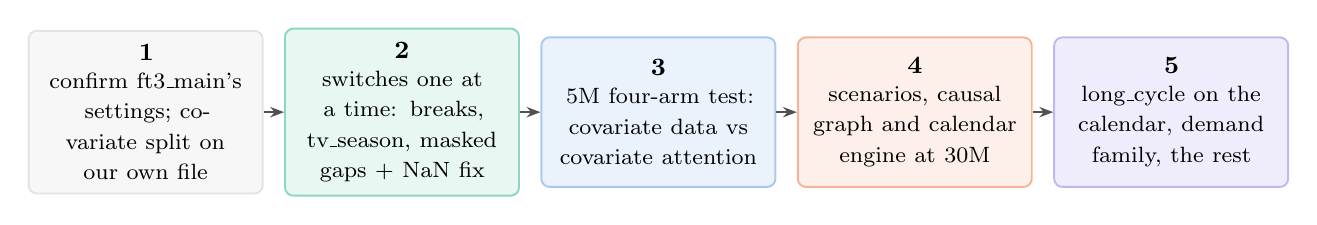
\begin{tikzpicture}[node distance=3mm and 2.6mm]
\node[gnode,text width=2.62cm,minimum height=1.9cm] (a) {\textbf{1}\\[-1pt]{\footnotesize confirm ft3\_main's settings; covariate split on our own file}};
\node[anode,right=of a,text width=2.62cm,minimum height=1.9cm] (b) {\textbf{2}\\[-1pt]{\footnotesize switches one at a time: breaks, tv\_season, masked gaps + NaN fix}};
\node[bnode,right=of b,text width=2.62cm,minimum height=1.9cm] (c) {\textbf{3}\\[-1pt]{\footnotesize 5M four-arm test: covariate data vs covariate attention}};
\node[onode,right=of c,text width=2.62cm,minimum height=1.9cm] (d) {\textbf{4}\\[-1pt]{\footnotesize scenarios, causal graph and calendar engine at 30M}};
\node[vnode,right=of d,text width=2.62cm,minimum height=1.9cm] (e) {\textbf{5}\\[-1pt]{\footnotesize long\_cycle on the calendar, demand family, the rest}};
\draw[arr] (a)--(b); \draw[arr] (b)--(c); \draw[arr] (c)--(d); \draw[arr] (d)--(e);
\end{tikzpicture}
\caption{Each step has a probe that isolates it, a dev-set score, and fev and TIME only at the end.}
\end{figure}

% =========================================================== 11
\section{Rules to keep}

\begin{keep}[Discipline]
\begin{enumerate}[leftmargin=16pt]
\item \textbf{Write the check before the run.} Hypothesis, the probe that isolates it, the dev datasets it should move, and the size of change that counts as a win.
\item \textbf{One change per fine-tune}, judged with paired confidence intervals.
\item \textbf{Keep the three data roles apart} (tuning, locked, final). Count every look at fev and TIME.
\item \textbf{Make sure our scorer reproduces 43.78.} The repository's scorer does not have the groups mode yet; until it does, a ``we beat X'' claim rests on a number the repository cannot regenerate.
\item \textbf{Record failures as carefully as successes.} The patch-probe and post-training notes are a good model.
\item \textbf{Decide the synthetic-only question now.} The top models post-train on real data. Choose whether ``synthetic only'' is part of the claim before the next results arrive, not after.
\end{enumerate}
\end{keep}

\begin{keep}[Usefulness, not just skill]
Skill is a geometric mean and hides the failures users notice. Report next to it: the share of windows more than twice as bad as Seasonal Naive, interval coverage at 80\% and 90\%, behaviour with missing values and outliers, stability when one new point arrives, whether covariates help or hurt, and speed per series.
\end{keep}

% =========================================================== 12
\section{Ideas worth exploring}

These are not yet in the plan. Each could become a probe or a generator family if the diagnosis points there.

\begin{explore}[More mathematical generators]
\begin{itemize}
\item \textbf{State-space and pole-zero sampling:} draw the roots of an ARMA or linear system directly to control cycles, damping and memory.
\item \textbf{Spectral-mixture Gaussian processes:} a few spectral peaks with widths give quasi-periodic structure in one draw.
\item \textbf{Point processes:} Hawkes, Cox and renewal processes for arrivals, bursts and call volumes.
\item \textbf{Stochastic differential equations with jumps:} Heston-style volatility, Merton jumps, fractional Brownian motion for long memory.
\item \textbf{Threshold and smooth-transition AR (TAR, STAR):} regimes that switch on the level itself.
\item \textbf{Multifractal and wavelet cascades:} bursty, self-similar traffic and turbulence.
\item \textbf{Dynamic factor models:} many series driven by a few shared factors, the natural shape of retail and macro panels.
\item \textbf{Observation operators:} censoring, aggregation, rounding, reporting delays and revisions applied after the process is drawn.
\end{itemize}
\end{explore}

\begin{explore}[Better ways to choose the mix]
\begin{itemize}
\item \textbf{Mixture search on the dev set (DoReMi-style):} learn family weights that reduce dev error, never benchmark error.
\item \textbf{Coverage maps:} compute features for real and synthetic windows; regions of real data with no synthetic neighbours name the missing family.
\item \textbf{A realism classifier:} a small model that tells real from synthetic windows; what it finds easy to spot is what the generator gets wrong.
\item \textbf{Quality-diversity search:} keep generator settings that are both realistic and different from each other.
\item \textbf{Oracle regret:} for families with a known best forecast (Kalman filter, GP posterior), measure how far the model is from the best possible answer.
\end{itemize}
\end{explore}

\begin{explore}[Questions for the paper]
\begin{itemize}
\item Does patch tokenisation gate in-context recall, and do the sub-patch dips follow the periods the training data over-represents? (A causal test: train with periods that avoid multiples of 4.)
\item How far can a synthetic-only model go when the covariate mechanisms are generated, not learned from real data?
\end{itemize}
\end{explore}

% =========================================================== appendix
\appendix
\section{Glossary and sources}

\begin{table}[H]
\centering\small
\begin{tabularx}{\linewidth}{>{\raggedright\arraybackslash\bfseries}p{3.4cm} Y}
\toprule
Skill score & $100\,(1-\text{geometric mean of } e_{\text{model}}/e_{\text{Seasonal Naive}})$ across tasks \\
MASE, CRPS & point error scaled by a naive forecast; error of the full predicted distribution \\
Covariate & another series that helps explain the target; known (future given) or past (history only) \\
Fixable error & our error minus the best reference model's error on the same window \\
Family & one kind of synthetic process in the generator (for example ets, repeat, long\_cycle) \\
Layer & a change applied on top of any family (seasonality, trend, calendar, noise, corruption) \\
Pass-through family & a family that skips the layers so its defining property survives (exact repetition, flatness) \\
Dev catalog & real datasets not in any benchmark, used for tuning and checking \\
CPM & contiguous patch masking: hiding a run of patches so the model learns to forecast several patches \\
\bottomrule
\end{tabularx}
\end{table}

{\sloppy\textbf{Sources.} fev-bench results: \texttt{github.com/autogluon/fev}, \texttt{benchmarks/fev\_bench/results} and \texttt{tasks.yaml}. TIME: \texttt{github.com/zqiao11/TIME}, \texttt{src/timebench/config/datasets.yaml}; paper arXiv 2602.12147 (dataset sources, Table 2). GIFT-Eval: \texttt{github.com/SalesforceAIResearch/gift-eval}. Project notes: TIME\_RESULTS, TIME\_FULL\_LEADERBOARD, TIMESTRAL\_GAP, PATCH\_PROBE, M4\_RESULTS, REAL\_POSTTRAIN\_RESULTS, DEV\_DATA\_CATALOG, GENERATOR\_GAPS. Generator: \texttt{tidemark/real/ft3\_core.py}.

\textbf{Files.} \texttt{make\_figs.py} (all figures), \texttt{gen\_audit.py} (generator measurements), \texttt{dataset\_catalog\_v2.csv}, \texttt{excluded\_benchmark.csv}, \texttt{benchmark\_datasets.csv}, \texttt{verify\_urls.py}.\par}

\end{document}
